% !TEX root = Master.tex

The same procedure as in Subsection \ref{sssec:margin_kcc_6} for key category cluster 2 is applied here to analyze the marginal distribution of the log-sales in key category cluster 6.\\

Excluding all covariates, simple maximum likelihood estimation results in parameters $\hat{\mu} = 9.62$, $\hat{\sigma} = 0.20$ and $\hat{\nu} = 0.41$ of the ex-Gaussian distribution.
\autoref{fig:kcc_6_density} shows the histogram of the observed log-sales along with a density curve fitted with the estimated parameters. A QQ-plot is displayed in \autoref{fig:kcc_6_qqplot}, where the data points match the line $y=x$ well, excluding a few outliers on the upper part of the plot.
 %can be summarized within \autoref{tab:estimated_parameters_kcc_6_no_covariates}, \autoref{fig:kcc_6_margin} and \autoref{fig:res_kcc_6_no_covariates}. 
 A Shapiro-Wilk test on the residuals returns a p-value of 0.87 and thus fails to reject the null hypothesis of non-normality. \autoref{fig:res_kcc_6_no_covariates} portrays a histogram of the residuals along with a density curve. Although it looks platykurtic to a certain extend, normality cannot be excluded as the Shapiro-Wilk test indicated.
\\


%
%\begin{table}[H]
%\setlength\arrayrulewidth{1pt}  
%\centering
%\begin{adjustbox}{max width=\textwidth}\
%\begin{tabular}{|c|c|c|}
%\hline
%\rowcolor{lightgray} 
%$\hat{\mu}$ & $\hat{\sigma}$ & $\hat{\nu}$ \\ \hline
%9.62        & 0.20           & 0.41        \\ \hline
%\end{tabular}
%\end{adjustbox}
%\caption{Estimated parameters for log-sales of KCC 6 fitted to ex-Gaussian distribution with no covariate effects}
%\label{tab:estimated_parameters_kcc_6_no_covariates}
%\end{table}



 \begin{figure}[H]
\centering
\begin{subfigure}{.45\textwidth}
  \centering
  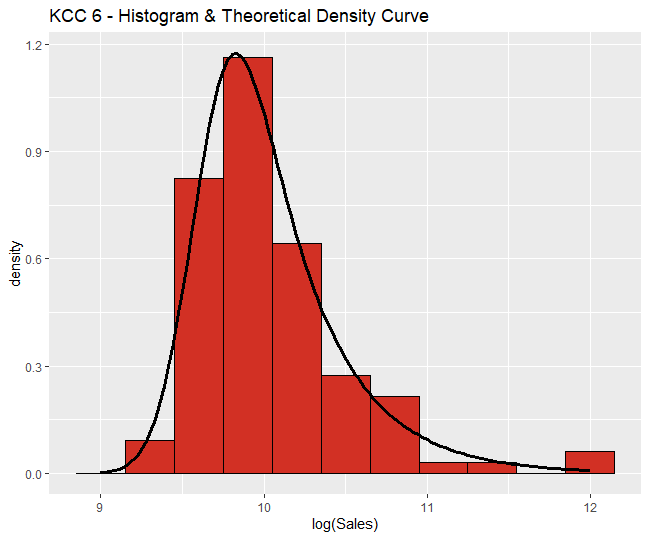
\includegraphics[width=\linewidth]{figures/kcc_6_density.png}
  \caption{Histogram \& theoretical density}
  \label{fig:kcc_6_density}
\end{subfigure}
\begin{subfigure}{.45\textwidth}
  \centering
  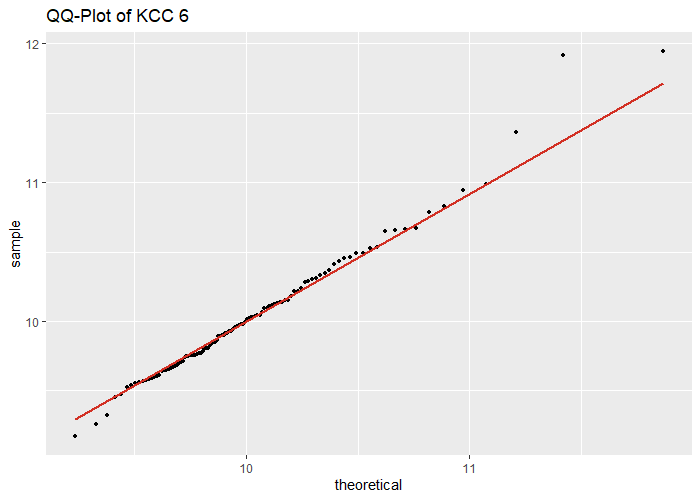
\includegraphics[width=\linewidth]{figures/kcc_6_qqplot.png}
  \caption{QQ-plot}
  \label{fig:kcc_6_qqplot}
\end{subfigure}
\caption{ex-Gaussian distribution fitted to log-sales of \ac{KCC} 6}
\label{fig:kcc_6_margin}
\end{figure} 


\begin{figure}[H]
\centering
  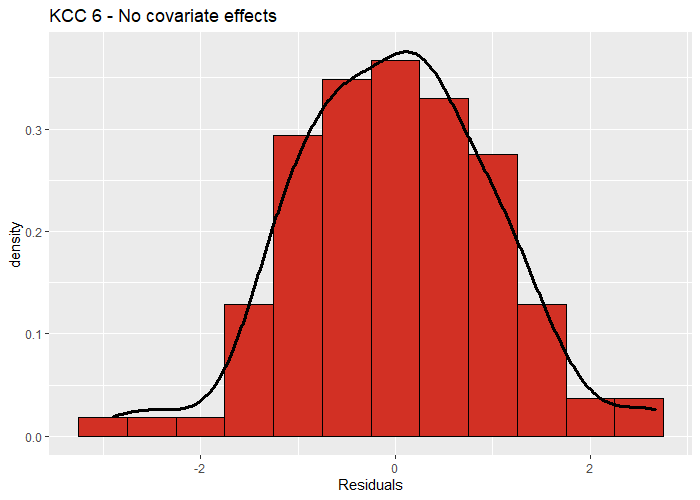
\includegraphics[width=0.45\linewidth]{figures/res_kcc_6_no_covariates.png}
  \caption{Residuals of KCC 6 log-sales fitted to an ex-Gaussian distribution with no covariate effects together with their density curve}
  \label{fig:res_kcc_6_no_covariates}
\end{figure}


Reviewing different model specifications, an equivalent model as in the previous Subsection is chosen (Model \ref{eq:gamlss_kcc_2}) with an ex-Gaussian distribution family for the response variable. The resulting parameter coefficients for $\hat{\mu}$ are printed in \autoref{tab:gamlss_coeff_kcc_6}, where we once again observe controversial results. A detailed summary of the model fit can be found in the \nameref{sec:appendix} (R output \ref{output:gamlss_fit_kcc_6_try1}). The two promotions seem to negatively interact with the total markdown percentage. Those kinds of behaviour might need further investigation.
The estimated time-varying location and scale parameters can be seen in \autoref{fig:gamlss_kcc_6_estimated_parameters} and the skewness parameter $\hat{\nu}$ with 95\% CI in \autoref{tab:nu_ci_kcc_6}. Fitted values are close to real values, capturing the promotion peaks fairly well. The standard deviation fluctuates throughout time within a range between 0.1 and 0.3.
\\


%\VerbatimInput[frame = single, label = "GAMLSS Fit on KCC 6" ]{gamlss_fit_kcc_6_try1.txt}



\begin{table}[H]
\centering
\begin{tabular}{l|c|c|c|l}
  \hline
  \rowcolor{white}
 \textbf{$\hat{\mu}$ Coefficients} & \textbf{Estimate} & \textbf{Std. Error} & \textbf{t value} & \textbf{p-value} \\ 
  \hline\hline
\textit{$\beta_{01}$ (Intercept)} & 8.31 & 0.11 & 71.80 & 0.00 *** \\ 
  \textit{$f_{11}$(time)} & 0.00 & 0.00 & 5.20 & 0.00 *** \\ 
  \textit{$f_{12}$(total\_markdown\_pct)} & 4.01 & 0.30 & 13.29 & 0.00 *** \\ 
  \textit{promo\_typeBlack Friday} & -0.81 & 0.30 & -2.73 & 0.01 ** \\ 
  \textit{promo\_typeFriends \& Family} & 0.87 & 0.48 & 1.81 & 0.07 . \\ 
  \textit{promo\_typeBlack Friday:total\_markdown\_pct} & 1.02 & 0.54 & 1.90 & 0.06 . \\ 
  \textit{promo\_typeFriends \& Family:total\_markdown\_pct} & -2.47 & 0.88 & -2.81 & 0.01 ** \\ \hline
\end{tabular}
\caption{Estimated $\hat{\mu}$ coefficients of \ac{GAMLSS} fit on log-sales of \ac{KCC} 6}
\label{tab:gamlss_coeff_kcc_6}
\end{table}





\begin{figure}[H]
\centering
  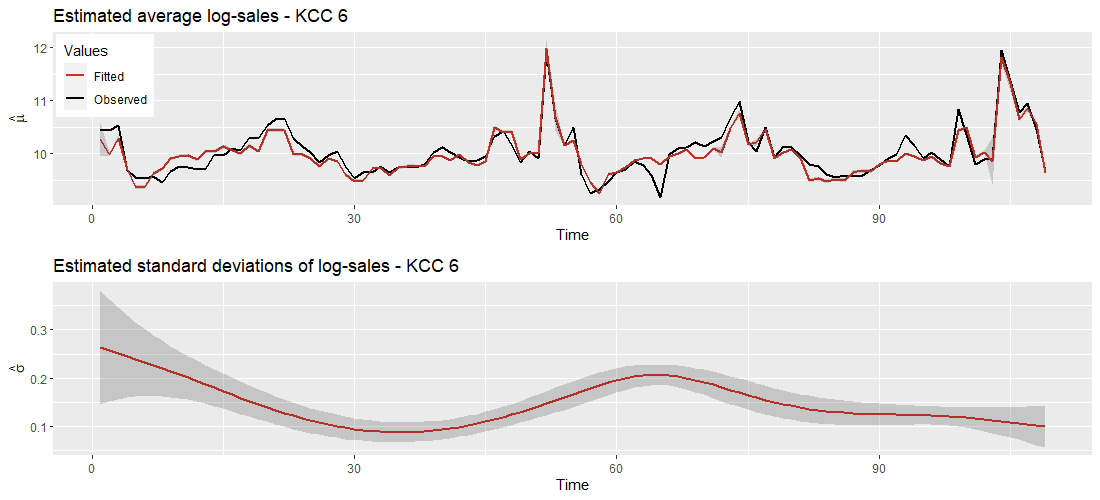
\includegraphics[width=0.95\linewidth]{figures/gamlss_kcc_6_estimated_parameters.png}
  \caption{Estimated location parameter $\hat{\mu}$ compared to the observed values and scale parameter $\hat{\sigma}$ with confidence bands of GAMLSS fit - KCC 6}
  \label{fig:gamlss_kcc_6_estimated_parameters}
\end{figure}



\begin{table}[H]
\setlength\arrayrulewidth{1pt}  
\centering
\begin{adjustbox}{max width=\textwidth}\
\begin{tabular}{c|c|c}
\hline
\rowcolor{white} 
\textbf{Lower} & $\hat{\nu}$ & \textbf{Upper} \\ \hline\hline
0.044        & 0.031           & 0.057        \\ \hline
\end{tabular}
\end{adjustbox}
\caption{Estimated skewness parameter $\hat{\nu}$ of GAMLSS fit with 95\% confidence interval bounds - KCC 6}
\label{tab:nu_ci_kcc_6}
\end{table}




\autoref{fig:gamlss_effects_kcc_6} reveals some interesting points regarding covariate effects. The temporal effect as well as the total markdown percentage collapse to increasing straight lines. 
%The temporal effect also exhibits symmetrical behaviour around zero, including uncertainty. 
%Just like in \ac{KCC} 2, the effect of Spring-Summer is slightly smaller than that of Fall-Winter.
As opposed to the \ac{GAMLSS} fit for \ac{KCC} 2, Friends \& Family seems to have the highest effect of all promos for this \ac{KCC}. 
\\



\begin{figure}[H]
\centering
  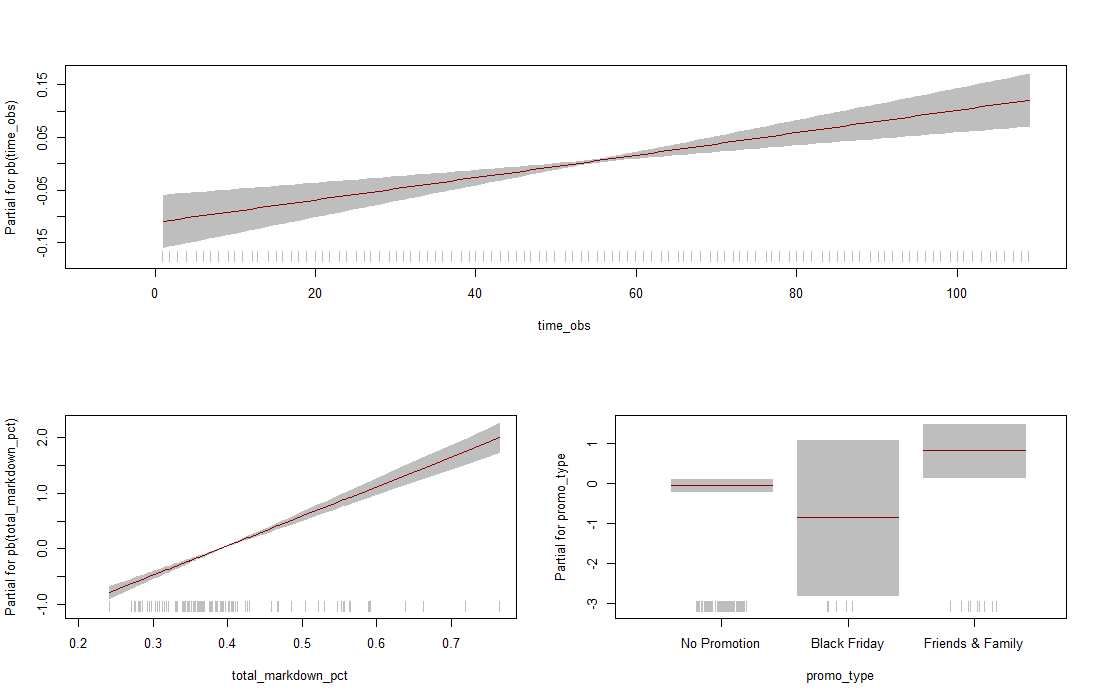
\includegraphics[width=0.95\linewidth]{figures/gamlss_effects_kcc_6.png}
  \caption{Covariate effects on the expected response variable (log-sales) of GAMLSS fit - KCC 6}
  \label{fig:gamlss_effects_kcc_6}
\end{figure}









\begin{figure}[H]
\centering
  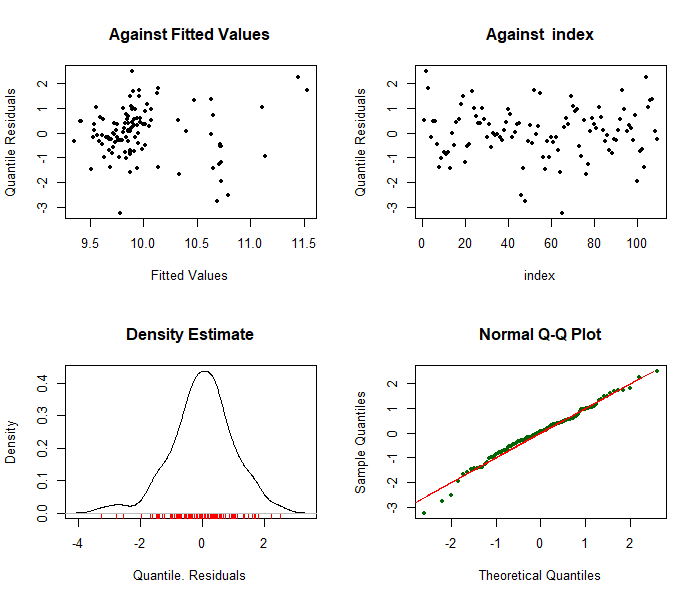
\includegraphics[width=0.95\linewidth]{figures/gamlss_residuals_kcc_6.png}
  \caption{Residuals of GAMLSS fit - KCC 6}
  \label{fig:gamlss_residuals_kcc_6}
\end{figure}


Inspecting the diagnostic plots for the residuals in \autoref{fig:gamlss_residuals_kcc_6} along with the associated summary in \autoref{tab:gamlss_residuals_kcc_6}, we can again confirm an appropriate fit. The plots in the upper row of \autoref{fig:gamlss_residuals_kcc_6} show how the points are scattered around (horizontal) zero without a clear pattern. The left lower plot resembles a normally distributed density curve adequately and the QQ-plot in the lower left corner displays the data matching to the diagona line. In \autoref{tab:gamlss_residuals_kcc_6}, metrics of the residuals are displayed. Those metrics indeed indicate an approximation of a standard normal distribution.  A Shapiro-Wilk test returns a p-value of 0.7, which is below the p-value of the fit without covariate effects. Nevertheless, normality is a steady assumption for the quantile residuals.
\\






\begin{table}[H]
\centering
\begin{tabular}{c}
\hline
\rowcolor{white} 
\textbf{Summary of the Quantile Residuals} \\ \hline\hline
 $\begin{array}[t]{ r @{{}={}} l }
\text{mean} & -0.01692598                         \\ 
\text{variance} & 1.011483                         \\ 
\text{coef. of skewness} & -0.1401063               \\ 
\text{coef. of kurtosis} & 3.144701                \\ \hline
\end{array}$
\end{tabular}
\caption{Residuals of GAMLSS Fit on KCC 2}
\label{tab:gamlss_residuals_kcc_6}
\end{table}


%\VerbatimInput[frame = single, label = "Residuals of GAMLSS Fit on KCC 6" ]{gamlss_residuals_kcc_6.txt}






%\inputRoutput[caption={Residuals of GAMLSS Fit on KCC 6},numbers=left,numberstyle=\tiny, label=output:gamlss_residuals_kcc_6]{gamlss_residuals_kcc_6.txt}
















